I'm not writing anything here since I hope that the code is self-explanatory.

I include only few figures to better understand results.

\begin{figure}[h!]
  \centering
  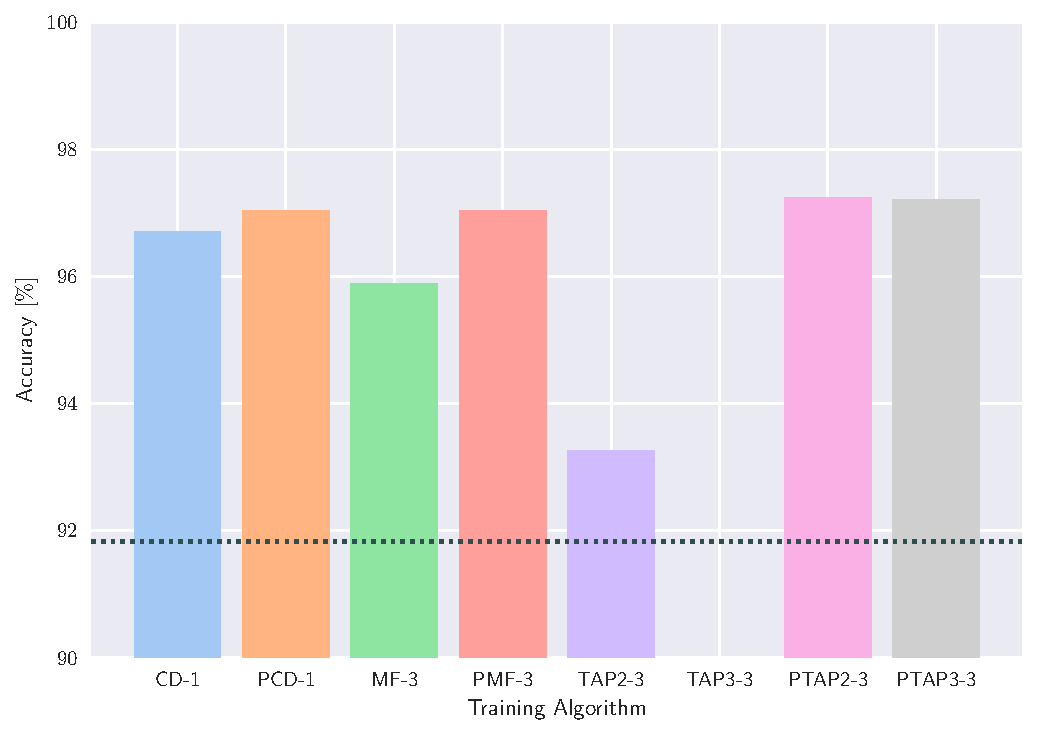
\includegraphics[width=0.6\textwidth]{img/numerical-experiments/acc-hist.pdf}
  \caption{accuracies of classification of MNIST images using hidden-layer activation probabilities. Logistic classifier was used; dashed line is pure classifier (without RBM)}
\end{figure}
\begin{figure}[h!]
  \centering
  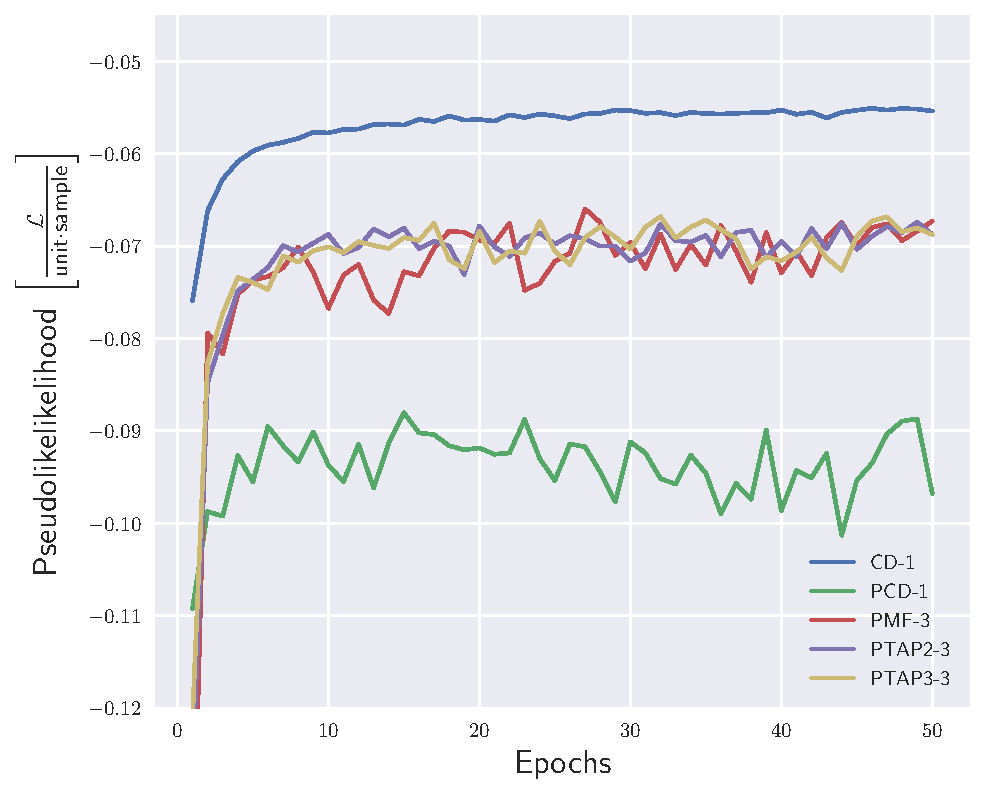
\includegraphics[width=0.6\textwidth]{img/numerical-experiments/psl-plot-global.pdf}
  \caption{pseudo-likelihood over epochs.}
\end{figure}